% !TEX root = atlas_iros_16.tex
%%%%%%%%%%%%%%%%%%%%%%%%%%%%%%%%%%%%%%%%%%%%%%%%%%%%%%%%%%%%%%%%%%%%%%%%%%%%%%%%
\section{\large Collision Detection}
\label{sec:CollDet}
%
In the following experiments (Sec.~\ref{sec:CollDet_EE} and \ref{sec:CollDet_Link}), we used the collision handling (\ref{eqn:CollDet}) and (\ref{eqn:CollReact}) to detect collisions with the Atlas robot with a disturbance joint torque threshold  $\bm{\zeta}$ of $11$~Nm for each joint.
A lower threshold frequently leads to false alarms due to remaining modeling errors (see Fig.~\ref{fig:ident_torque_compare}) and the large friction effects (see Fig.~\ref{fig:ident_friction_char}).
Our model is not able to reliably remove the static friction torque from the observer ($\kappa_{\mathrm{f}}=1$ in (\ref{eqn:observer_settings})) due to the indeterminate friction state for low velocities \cite{BidardLibArhMea2005}.
The friction compensation in (\ref{eqn:controller}) currently leads to unwanted oscillations indicating closed-loop stability problems originating in the velocity feedback, as described in \cite{ConnerKohRomStu2015}.
Therefore, this feature is disabled in the experiments with $\kappa_{\mathrm{f}}=0$. 
However, it is possible to reliably detect soft collisions at moderate velocity (100~mm/s) in adequate time with the Atlas system.
For the collision detection and reaction experiments, the disturbance compensation in (\ref{eqn:controller}) was disabled ($\kappa_\varepsilon=0$).
The first joint was selected for evaluation of the experiments, since the collision is detected at this joint first. The other axes show qualitatively the same behavior.

\subsection{End-effector Collision}
\label{sec:CollDet_EE}
%
\begin{figure}
\begin{subfigure}{.24\textwidth}
  \centering
  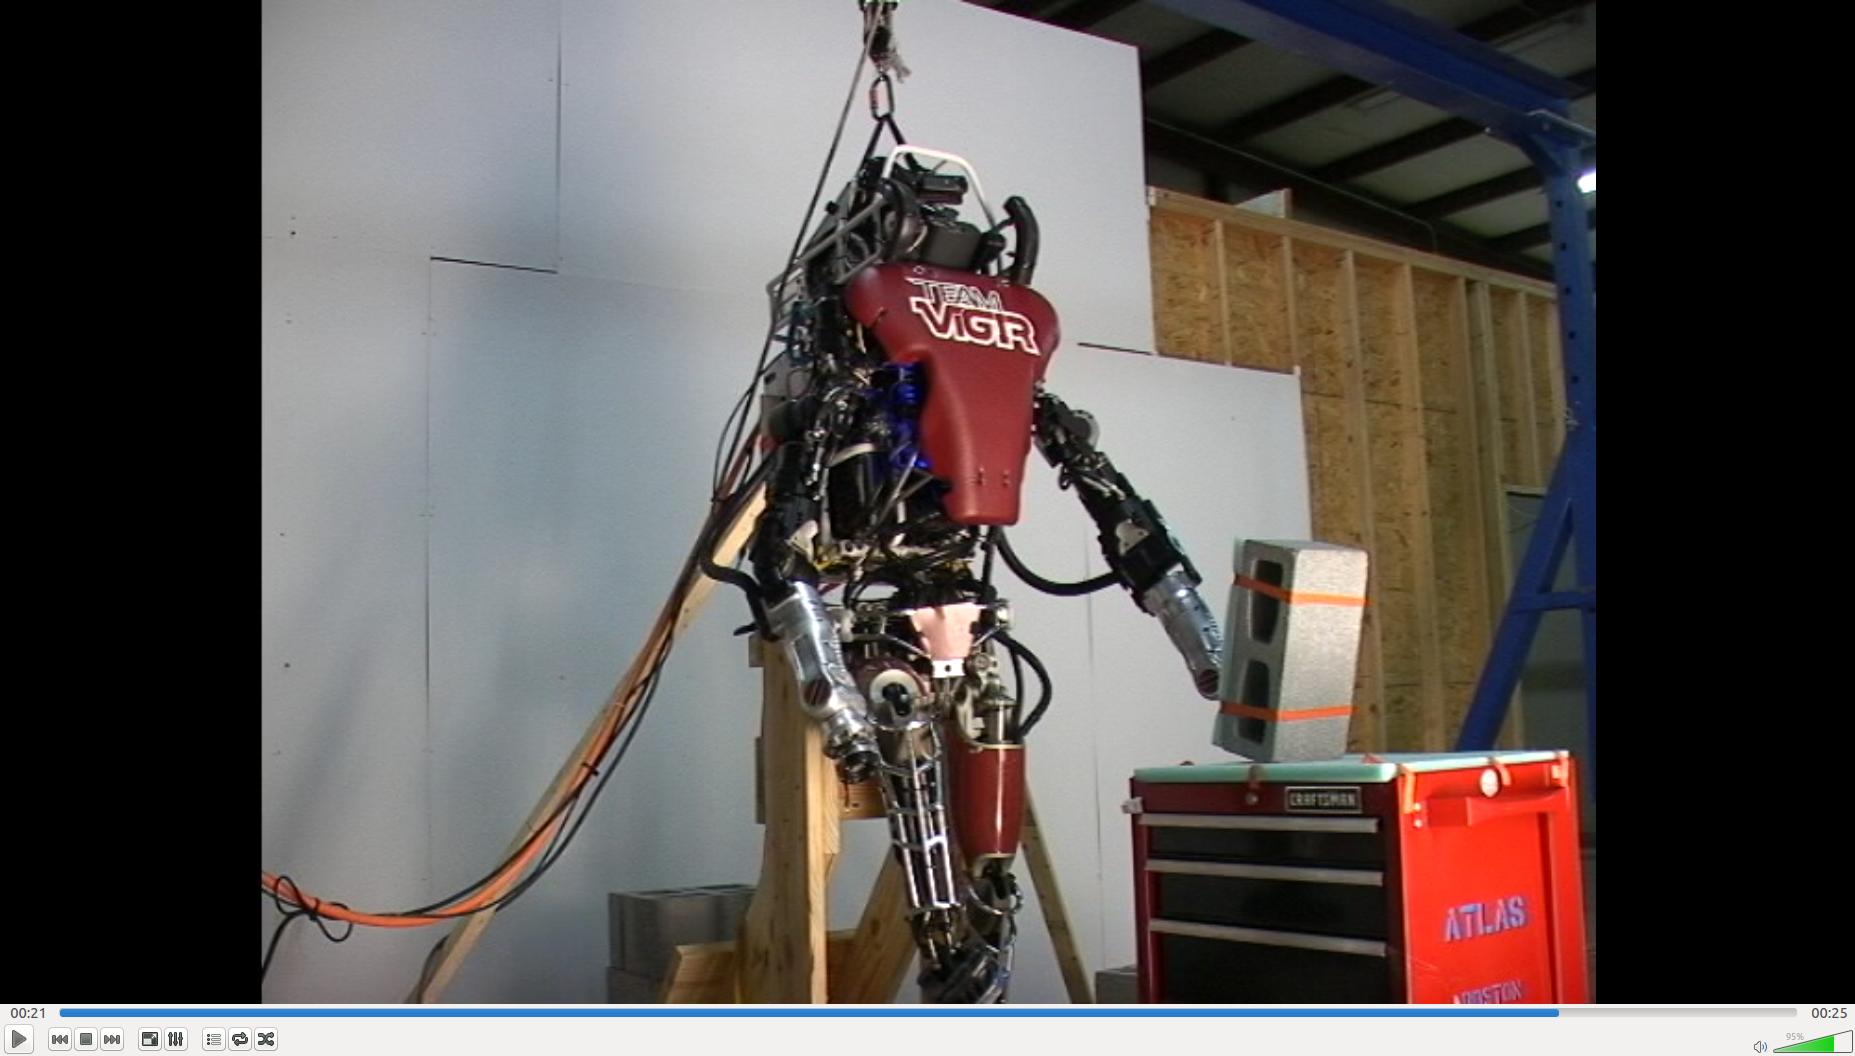
\includegraphics[trim=550 250 350 100,clip,width=.98\linewidth]{figures/CollDetCinderblock/ImpCtrlv5_E057_R04_impCtrl_K300_wall_colldet_move_away_021.jpg}
  \caption{Enabled (``Coll.Det'' in Fig.~\ref{fig:CinderCollisionSummary})}
  \label{fig:CinderColl_zerog}
\end{subfigure}%
\begin{subfigure}{.24\textwidth}
  \centering
  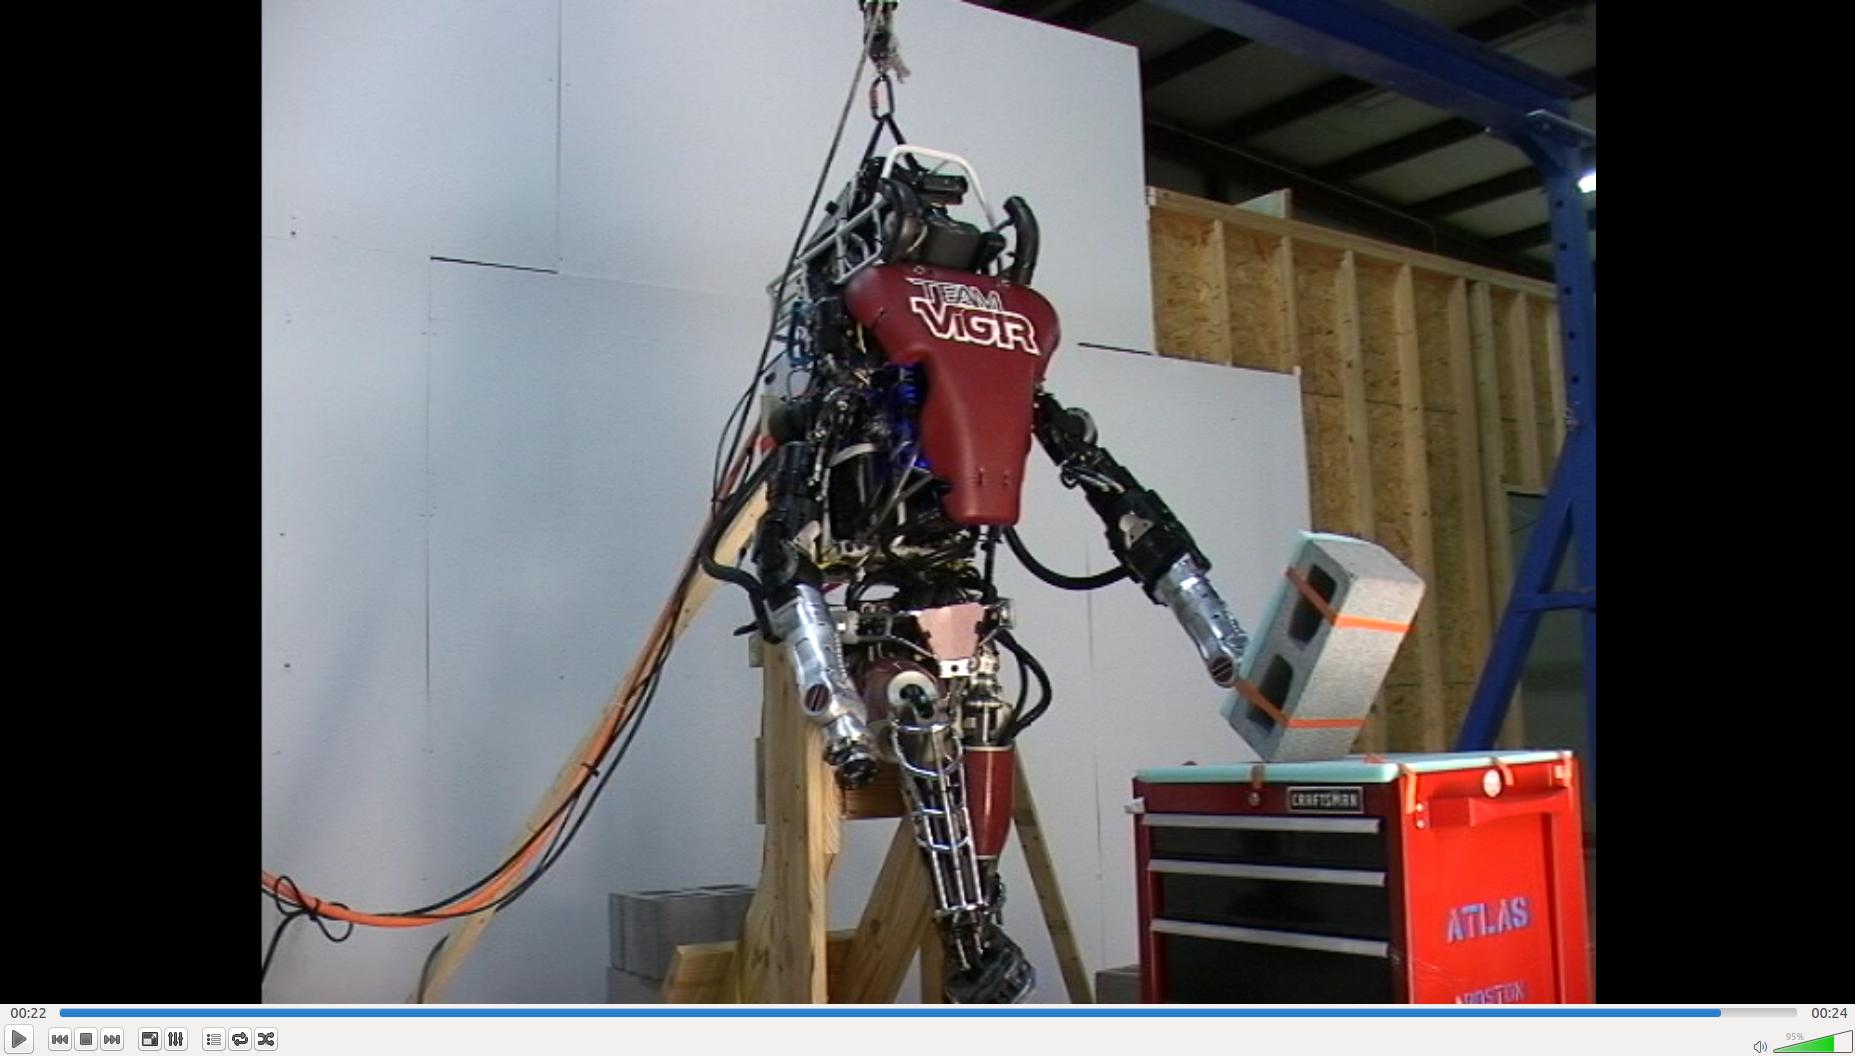
\includegraphics[trim=550 250 350 100,clip,width=.98\linewidth]{figures/CollDetCinderblock/ImpCtrlv5_E057_R05_impCtrl_K300_wall_nocolldet_collision_022.jpg}
  \caption{Disabled (``Stiff'' in Fig.~\ref{fig:CinderCollisionSummary})}
  \label{fig:CinderColl_push}
\end{subfigure}
\caption{Result after the end-effector collision with and without detection and reaction (snapshot at $t\approx1.5$~s of Fig.~\ref{fig:CinderCollisionSummary})}
\label{fig:CinderCollPictures}
\SkipBeforeText
\end{figure}
%
\begin{figure}
\centering
\parbox{\columnwidth}{
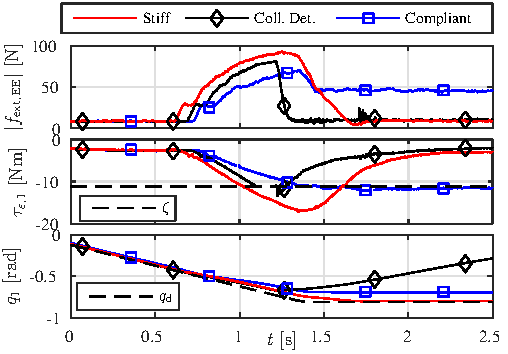
\includegraphics{figures/CollDetCinderblock/Collision_Summary_Cinderblock.pdf}
}
\vspace*{-1ex}
\caption{Absolute external force $|\bm{f}_\mathrm{ext,EE}|$, observed disturbance torque $\hat{\tau}_{\varepsilon,1}$ and joint position $q_1$ are depicted for the cinderblock collision experiment (see also Fig.~\ref{fig:CinderCollPictures}).
For the ``Stiff'' and ``Coll.Det'' mode, $k_i=300$~Nm/rad and for the ``Compliant'' mode $k_i=100$~Nm/rad were chosen.}
\label{fig:CinderCollisionSummary}
\SkipBeforeText
\end{figure}
%
The first experiment lets the end-effector collide with a styrofoam-protected cinderblock, see Fig.~\ref{fig:CinderCollPictures}.
The protection aimed to protect the robot from damage and has no major influence on the collision detection.
The measured data during the three runs with different settings is depicted in Fig.~\ref{fig:CinderCollisionSummary}.
Using a rather stiff joint impedance controller with joint-wise $k_i=300$~Nm/rad  (``Stiff'') and deactivated collision handling leads to pushing the cinderblock away and tipping it over till reaching the final goal position, see Fig.~\ref{fig:CinderCollPictures}~(b) and Fig.~\ref{fig:CinderCollisionSummary}.
Reducing the joint stiffness to \mbox{$k_i=100$~Nm/rad} (``Compliant'') leads to smaller resulting quasi-static contact forces, while the positioning error increases, see Fig.~\ref{fig:CinderCollisionSummary}.

Using the collision detection and reaction (``Col. Det.''), the arm drifts away after the collision has been detected and the contact force decays to zero, see Fig.~\ref{fig:CinderCollPictures}~(a) and Fig.~\ref{fig:CinderCollisionSummary}.
The collision in Fig.~\ref{fig:CinderCollisionSummary} is detected at $t=1.1$~s, when the disturbance torque line crosses the detection threshold $\bm{\zeta}$.
At this point in time, the maximum contact force of about 69~N is already reached, which is caused by the relatively slow dynamics of the observer (\mbox{$k_{\mathrm{o},i}=5~\mathrm{s}^{-1}$}).
A larger gain would allow an earlier detection with less reaction force.
Using retract reflexes would allow further reduction of contact forces.
In turn, larger observer gain causes vibrations when being used as disturbance compensation.
To overcome this issue, two observers could be used in parallel: a slower one for compensation and a faster one for collision detection.

\subsection{Link Collision}
\label{sec:CollDet_Link}
%
\begin{figure}
\centering
\parbox{\columnwidth}{
% 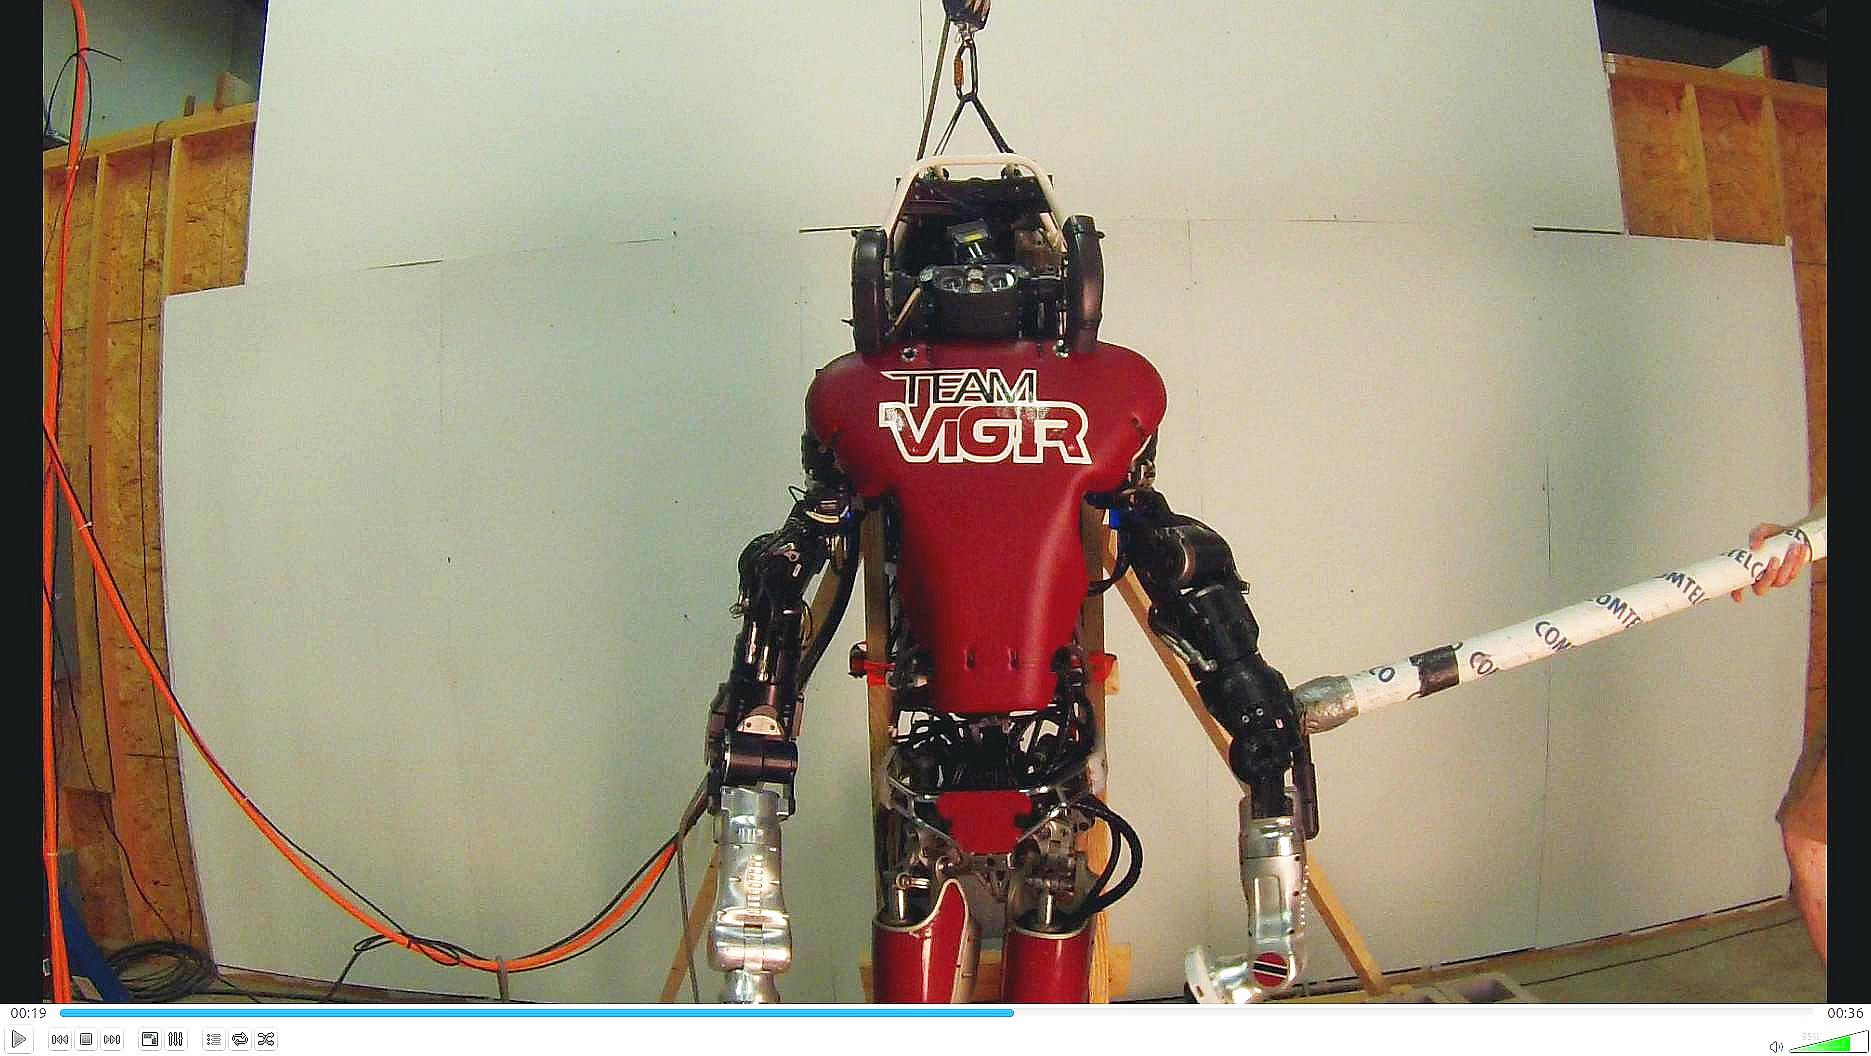
\includegraphics[trim=550 50 350 340,clip,width=\linewidth]{figures/CollDetStick/GOPR2201_ImpCtrlv5_E055_part4_t036.jpg}
\input{./figures/CollDetStick/GOPR2201_ImpCtrlv5_E055_part4_t036_bearb.pdf_tex}
}
\caption{Scene during the collision from Fig.~\ref{fig:StickCollisionSummary} at $t\approx5.5$~s.}
\label{fig:StickCollisionPhoto}
\SkipBeforePicture
\end{figure}
%
\begin{figure}
\centering
\parbox{\columnwidth}{
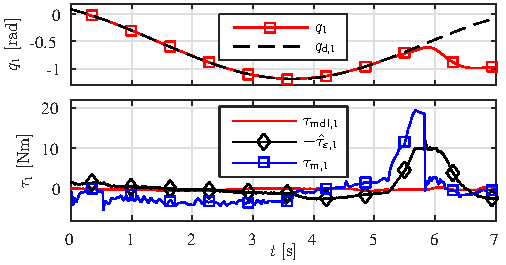
\includegraphics{figures/CollDetStick/CollDetStickIROS.pdf}
}
\vspace*{-1ex}
\caption{Joint position $q_1$, model torque $\tau_{\mathrm{mdl},1}$, estimated disturbance torque $\hat{\tau}_{\varepsilon,1}$ and motor-side joint torque $\tau_{\mathrm{m},1}$ during link collision, see Fig.~\ref{fig:StickCollisionPhoto}.}
\label{fig:StickCollisionSummary}
\SkipBeforeText
\end{figure}
%
The second experiment shows that collisions at the proximal links and not only at the end-effector are detected as well.
The arm was pushed at the elbow with a cardboard stick against the moving direction during a joint trajectory, see Fig.~\ref{fig:StickCollisionPhoto} (in the depicted situation, the elbow was moving to the right).
The movement speed was $\approx50~\mathrm{mm/s}$ at the collision location.
Figure~\ref{fig:StickCollisionSummary} depicts the measurement data. The collision at link $4$ starts at $t\approx5.5$~s, which one can see from the high motor torque in joint 1.
The detection threshold is reached at $t\approx5.6$~s, leading to the halt in gravity compensation mode.

